\def\i{\item}
\graphicspath{{../pictures/vande28/}}
\chapter{Chương 5}
\section{Điểm. Đường thẳng. Tia. Đoạn thẳng.}
\subsection{Kiến thức cơ bản}
\immini{\subsubsection{Điểm}
	\begin{enumerate}[--,leftmargin=*]
		\i Là dấu chấm nhỏ trên giấy.                                                    
		\i Dùng chữ cái in hoa để đặt tên điểm, chẳng hạn $A,B,M,\ldots$  
\end{enumerate}}{
	\begin{tikzpicture}
	\filldraw [black] (0,0) circle [radius=2pt] node[left] {$A$};
	\filldraw [black] (2.5,0.2) circle [radius=2pt] node[right] {$B$};
	\filldraw [black] (1.5,1.5) circle [radius=2pt] node[above] {$C$};
	\end{tikzpicture}	
}
\subsubsection{Đường thẳng}
\begin{enumerate}[--,leftmargin=*]
	\i Đường thẳng không bị giới hạn 2 phía.
	\i Dùng chữ cái thường để đặt tên đường thẳng chẳng hạn: $a,b,c,\ldots$
\begin{center}
	\begin{tikzpicture}
		\draw (-4,0) -- (0,0) (-4,2) -- (0,1);
		\node at (-2.3,2) {$a$};
		\node at (-3,0.5) {$b$};
	\end{tikzpicture}
\end{center}
\i Điểm $M$ nằm trên đường thẳng $d$, ta nói điểm $M$ thuộc đường thẳng $d$. Kí hiệu $M\in d.$
\begin{center}
	\begin{tikzpicture}
		\draw(-4,0) -- (0,0);
		\filldraw[black] (-2,0) circle [radius = 2pt] node[above right] {$M$};
		\filldraw[black] (-2,1) circle [radius = 2pt] node[above left] {$N$};
		\node at (-3.5,0.2) {$d$};
	\end{tikzpicture}
\end{center}
\i Điểm $N$ không nằm trên đường thẳng $d$, ta nói $N$ không thuộc $d$. Kí hiệu $N\notin d.$
\end{enumerate}
\subsubsection{Ba điểm thẳng hàng}
Ba điểm thẳng hàng là ba điểm cùng thuộc một đường thẳng 
\begin{center}
	
\begin{tikzpicture}
		\filldraw[black] (0,0) circle[radius = 2pt] node[above] {$A$};
		\filldraw[black] (2,0) circle[radius = 2pt] node[above] {$B$};
		\filldraw[black] (4,0) circle[radius = 2pt] node[above] {$C$};
		\node at (-1, 0.3) {$a$};
		\draw (-2,0) -- (6,0);
	\end{tikzpicture}
\end{center}
\subsubsection{Hai đường thẳng song song, cắt nhau, trùng nhau}
\begin{center}
	\begin{tabularx}{\textwidth}{|*{3}{Y|} }
		\hline
		Hai đường thẳng song song&	Hai đường thẳng cắt nhau&	Hai đường thẳng trùng nhau\\
		\hline
		Là hai đường thẳng không có điểm chung.& Là hai đường thẳng có duy nhất một điểm chung. & Là hai đường thẳng có vô số điểm chung.\\
		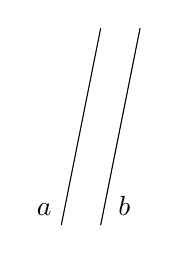
\begin{tikzpicture}
			\draw (0,0) -- (0.5,2.5) (0.5,0) --(1,2.5);
			\draw (0,0) node [above left] {$a$};
			\draw (0.6,0) node [above right] {$b$};
		\end{tikzpicture} &
		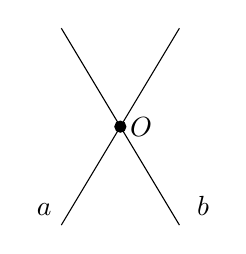
\begin{tikzpicture}
			\draw (0,0) --(1.5,2.5)  (0, 2.5) -- (1.5, 0);
			\draw (0,0) node [above left] {$a$};
			\draw (1.6,0) node [above right] {$b$};
			\filldraw[black] (0.75,1.25) circle[radius = 2pt] node[right] {$O$};
		\end{tikzpicture}&  
		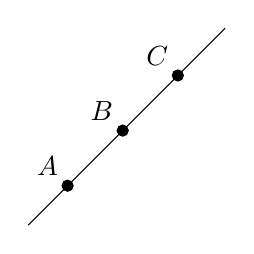
\begin{tikzpicture}
			\draw (0,0) -- (2.5,2.5);
			\filldraw[black] (0.5,0.5) circle [radius = 2pt] node [above left ]{$A$};
			\filldraw[black] (1.2,1.2) circle [radius = 2pt] node [above left ]{$B$};
			\filldraw[black] (1.9,1.9) circle [radius = 2pt] node [above left ]{$C$};
		\end{tikzpicture}\\
		Hai đường thẳng $a$ và $b$ song song.
		Kí hiệu: $a//b$ & Đường thẳng $a,b$ cắt nhau tại $O$. & Đường thẳng $AB,BC$ trùng nhau.\\
		\hline
	\end{tabularx}
\end{center}
\subsubsection{Tia}
\begin{enumerate}[--,leftmargin=*]
\i Hình gồm điểm $O$ và một phần đường thẳng bị chia ra bởi điểm $O$ được gọi là một tia gốc $O$. 
Điểm $O$ là gốc của tia.	
\begin{center}
	\begin{tikzpicture}
		\draw (0,0) -- (4,0);
		\draw (0,0.1) -- (0, -0.1);
		\draw (0, 0.5) node {$O$};
		\draw (4, 0.5) node {$x$};
		\draw (2, -0.5) node{Tia $Ox$.};
	\end{tikzpicture}
\end{center}
\i Hai tia đối nhau là 2 tia chung gốc và tạo thành đường thẳng.
\begin{center}
	\begin{tikzpicture}
		\draw (-4,0) -- (4,0);
		\draw (0,0.1) -- (0, -0.1);
		\draw (0, 0.5) node {$O$};
		\draw (4, 0.5) node {$x$};
		\draw (-4, 0.5) node {$y$};
		\draw (0, -0.5) node{Hai tia $Ox,Oy$ đối nhau.};
	\end{tikzpicture}
\end{center}

\end{enumerate}
\subsubsection{Đoạn thẳng}
Đoạn thẳng $AB$ hay đoạn thẳng $BA$ là hình gồm 2 điểm$ A,B$ cùng với các điểm nằm giữa$ A$ và $B$
\begin{center}
	\begin{tikzpicture}
		\draw (-4,0) -- (0,0)(0,0.1) -- (0, -0.1) (-4,0.1) -- (-4, -0.1);
		\draw (-4,0) node[above] {$A$};
		\draw (0,0) node[above] {$B$};
	\end{tikzpicture}
\end{center}
-- $A,B$ là hai đầu mút của đoạn thẳng.
\subsection{Thực hành giải toán.}
\begin{vd}
	Trong hình vẽ dưới đây, điểm nào thuộc đường thẳng $d$, điểm nào không thuộc đường thẳng $d$ (ghi bằng kí hiệu).
	\begin{center}
		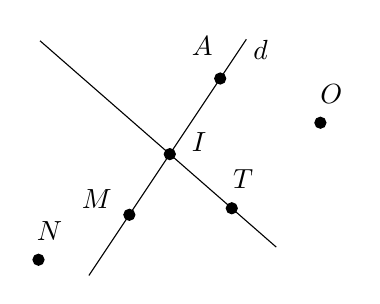
\begin{tikzpicture}
			\draw (-1.,1.)-- (1.,4.);
			\draw (-1.62,3.98)-- (1.38,1.36);
				\draw[color=black] (1.18,3.87) node {$d$};
				\draw [fill=black] (0.027471910112359645,2.5412078651685395) circle (2pt);
				\draw (0.4,2.69) node {$I$};
				\draw [fill=black] (-0.48615384615384605,1.7707692307692309) circle (2pt);
				\draw[color=black] (-0.9,1.97) node {$M$};
				\draw [fill=black] (0.6676923076923078,3.5015384615384617) circle (2pt);
				\draw[color=black] (0.44,3.91) node {$A$};
				\draw [fill=black] (0.8145830917021759,1.8537974332467664) circle (2pt);
				\draw[color=black] (0.96,2.23) node {$T$};
				\draw [fill=black] (-1.64,1.2) circle (2pt);
				\draw (-1.5,1.57) node {$N$};
				\draw [fill=black] (1.94,2.94) circle (2pt);
				\draw (2.08,3.31) node {$O$};
		\end{tikzpicture}
	\end{center}
	\loigiai{
		$A\in d;M\in d;I\in d.$
		
		$T\notin d;O\notin d;N\notin d.$
	}
\end{vd}
\begin{vd}
	Trong hình dưới đây có bao nhiêu đường thẳng? Em hãy đọc tên các đường thẳng đó.
	\begin{center}
		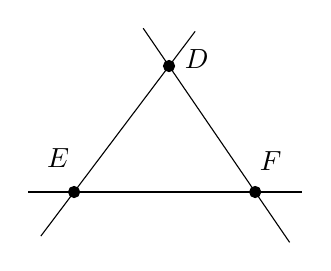
\begin{tikzpicture}
			\draw  (-0.64,4.66)-- (-2.6,2.06);
			\draw  (-2.76,2.62)-- (0.72,2.62);
			\draw  (0.56,1.98)-- (-1.3,4.7);

			\draw [fill=black] (-0.9717302698874813,4.219949641985994) circle (2.0pt);
			\draw[color=black] (-0.62,4.31) node {$D$};
			\draw [fill=black] (-2.1778461538461547,2.62) circle (2.0pt);
			\draw[color=black] (-2.38,3.05) node {$E$};
			\draw [fill=black] (0.1223529411764706,2.62) circle (2.0pt);
			\draw[color=black] (0.32,3.01) node {$F$};
		\end{tikzpicture}
	\end{center}
	\loigiai{
		Có 3 đường thẳng $DE,DF,EF$.}
\end{vd}
\begin{vd}
	Kể tên bộ 3 điểm thẳng hàng 
	\begin{center}
		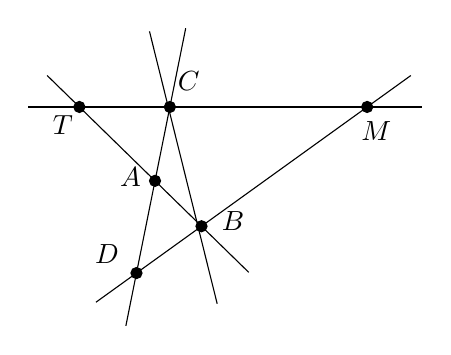
\begin{tikzpicture}
			\draw  (-3.,3.)-- (2.,3.);
			\draw  (-1.,4.)-- (-1.76,0.22);
			\draw  (-2.14,0.52)-- (1.86,3.4);
			\draw  (-2.76,3.4)-- (-0.2,0.9);
			\draw  (-0.6,0.5)-- (-1.46,3.96);
		
				\draw [fill=black] (-0.7993295266163197,1.48528274083625) circle (2.0pt);
				\draw[color=black] (-0.4,1.55) node {$B$};
				\draw [fill=black] (-2.3504,3.) circle (2.0pt);
				\draw[color=black] (-2.56,2.77) node {$T$};
				\draw [fill=black] (-1.2010582010582014,3.) circle (2.0pt);
				\draw[color=black] (-0.96,3.33) node {$C$};
				\draw [fill=black] (1.3044444444444445,3.) circle (2.0pt);
				\draw[color=black] (1.42,2.69) node {$M$};
				\draw [fill=black] (-1.3896897242761386,2.0618063713634167) circle (2.0pt);
				\draw[color=black] (-1.7,2.11) node {$A$};
				\draw [fill=black] (-1.6251521900519676,0.8906904231625834) circle (2.0pt);
				\draw[color=black] (-2.,1.13) node {$D$};
		\end{tikzpicture}
	\end{center}                       
	\loigiai{$(T,C,M);(T,A,B);(C,A,D);(M,B,D).$} 
\end{vd}
\begin{vd}
	Thực hành vẽ.
	\begin{enumerate}[a),leftmargin=*]
		\i Vẽ điểm $A\in d,B\notin d.$
		\i Điểm $M$ nằm giữa 2 điểm $A,B$.\\
		Điểm $N$ không nằm giữa $A,B$ (3 điểm$ A,B,N$ thẳng hàng).
		\i Ba điểm $M,N,P$ thẳng hàng; $M,N$ nằm cùng phia với$P$.
		\i Hai điểm $O,P$ nằm cùng phía với $Q$ nhưng $P$ không nằm giữa $O$ và $Q$.
		\i Vẽ 2 đường thẳng $AB,CD$ cắt nhau tại $I $(điểm $I\ne A,B,C,D$)
		\i Vẽ hai đường thẳng $AB,CD$ cắt nhau tại$A$.
		\i Vẽ tia $Ox$, trên $Ox$ lấy điểm $A$.\\
		Vẽ tia $Oy$ là tia đối của tia $Ox$, trên $Oy$ lấy điểm $B$. 
	\end{enumerate}   
	\loigiai{
		\begin{enumerate}[a),leftmargin=*]
		\i\hspace*{150pt}\begin{tikzpicture}
				\draw (0,0) -- (4,0);
				\filldraw[black] (1,0) circle[radius = 2pt] node[above] {$A$};
				\filldraw[black] (3,1) circle[radius = 2pt] node[above] {$B$};
				\draw (4, 0.5) node {$d$};
			\end{tikzpicture}
		
		\i\hspace*{150pt}
			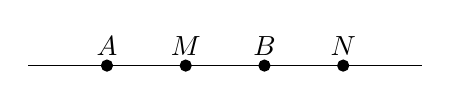
\begin{tikzpicture}
				\draw (0,0) -- (5,0);
				\filldraw[black] (1,0) circle[radius = 2pt] node[above] {$A$};
				\filldraw[black] (2,0) circle[radius = 2pt] node[above] {$M$};
				\filldraw[black] (3,0) circle[radius = 2pt] node[above] {$B$};
				\filldraw[black] (4,0) circle[radius = 2pt] node[above] {$N$};
			\end{tikzpicture}
		\i \hspace*{150pt}
			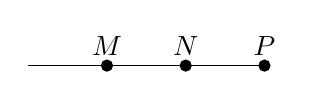
\begin{tikzpicture}
				\draw (0,0) -- (3,0);
				\filldraw[black] (1,0) circle[radius = 2pt] node[above] {$M$};
				\filldraw[black] (2,0) circle[radius = 2pt] node[above] {$N$};
				\filldraw[black] (3,0) circle[radius = 2pt] node[above] {$P$};
			\end{tikzpicture}
		\i \hspace*{150pt}
			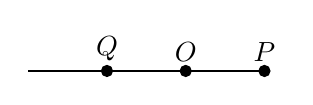
\begin{tikzpicture}
				\draw (0,0) -- (3,0);
				\filldraw[black] (1,0) circle[radius = 2pt] node[above] {$Q$};
				\filldraw[black] (2,0) circle[radius = 2pt] node[above] {$O$};
				\filldraw[black] (3,0) circle[radius = 2pt] node[above] {$P$};
			\end{tikzpicture}
	\i \hspace*{150pt}
		\begin{tikzpicture}
			\draw  (-1.58,3.38)-- (1.64,1.58);
			\draw  (-2.,1.54)-- (1.44,3.44);
				\draw [fill=uuuuuu] (-0.1330664500406172,2.571155158407799) circle (2.0pt);
				\draw[color=uuuuuu] (0.,2.91) node {$I$};
				\draw [fill=xdxdff] (-1.010317157050057,3.0615437523882307) circle (2pt);
				\draw[color=xdxdff] (-0.88,3.43) node {$A$};
				\draw [fill=xdxdff] (1.0210058493283563,1.9260215749096143) circle (2pt);
				\draw[color=xdxdff] (1.16,2.29) node {$B$};
				\draw [fill=xdxdff] (0.8686119816623066,3.124407780569297) circle (2pt);
				\draw[color=xdxdff] (1.,3.49) node {$C$};
				\draw [fill=xdxdff] (-1.231437229661478,1.9644968789660442) circle (2pt);
				\draw[color=xdxdff] (-1.1,2.33) node {$D$};
		\end{tikzpicture}
	\i \hspace*{150pt}
	\begin{tikzpicture}
			\draw  (-0.98,3.22)-- (2.24,1.42);
			\draw  (-2.,1.54)-- (1.44,3.44);

				\draw [fill=uuuuuu] (0.024765556458164254,2.6583298131600324) circle (2.0pt);
				\draw[color=uuuuuu] (0.06,3.13) node {$A$};
				\draw [fill=xdxdff] (1.6210058493283568,1.7660215749096144) circle (2.pt);
				\draw[color=xdxdff] (1.76,2.13) node {$B$};
				\draw [fill=xdxdff] (0.8686119816623066,3.124407780569297) circle (2.pt);
				\draw[color=xdxdff] (1.,3.49) node {$C$};
				\draw [fill=xdxdff] (-1.231437229661478,1.9644968789660442) circle (2.pt);
				\draw[color=xdxdff] (-1.1,2.33) node {$D$};
	\end{tikzpicture}
	\i \hspace*{150pt}
	\begin{tikzpicture}
		\draw (-4,0) -- (4,0);
		\draw (-0.1, 0) -- (0.1,0);
		\filldraw[black] (-2,0) circle[radius = 2pt] node[above] {$B$};
		\filldraw[black] (2,0) circle[radius = 2pt] node[above] {$A$};
		\draw(-4,0) node[above] {$y$};
		\draw(4,0) node[above] {$x$};
		\draw(0,0.2) node[above] {$O$};
	\end{tikzpicture}
	\end{enumerate}
	}
\end{vd}
\begin{vd}
	Cho 10 điểm trong đó không có 3 điểm nào thẳng hàng. Nối 2 điểm tạo thành một đường thẳng. Tính số đường thẳng tạo thành từ 2 trong 10 điểm đã cho?
	\loigiai{
		Vì cứ  qua 2 điểm ta kẻ đường thẳng nên mỗi điểm ta sẽ nối được với 9 điểm còn lại tạo thành 9 đường thẳng		
		Khi đó số đường thẳng tạo thành từ 2 trong 10 điểm đã cho là: $\frac{10\cdot9}{2}=45$ đường thẳng  (do số đường thẳng bị trùng)
	}
\end{vd}
\subsection{Mở rộng kiến thức}
\subsubsection{Hai tia trùng nhau}
\begin{enumerate}[--,leftmargin=*]
\i Hai tia trùng nhau: Là hai tia chung gốc và có thêm ít nhất một điểm chung khác nữa là hai tia trùng nhau.	
\begin{center}
	\begin{tikzpicture}
		\draw (-4,0) --(4,0) (0, 0.1) --(0, -0.1) (4,0.1) --(4, -0.1) (-4,0.1) --(-4, -0.1);
		\draw (-4,0) node[above] {$O$};
		\draw (0,0) node[above] {$A$};
		\draw (4,0) node[above] {$B$};
	\end{tikzpicture}
\end{center}
$OA,OB$ là hai tia trùng nhau.
\i Hai tia không trùng nhau được gọi là hai tia phân biệt.
\end{enumerate}
\subsubsection{Công thức tính số đường thẳng, số đoạn thẳng tạo thành.}
\begin{enumerate}[--,leftmargin=*]
\i Cho $n$ điểm trong đó không có 3 điểm nào thẳng hàng. Nối 2 điểm tạo thành một đường thẳng. Mỗi điểm ta sẽ nối được với $n-1$ điểm còn lại tạo thành $n-1$ đường thẳng.
Khi đó số đường thẳng tạo thành từ 2 trong $n$ điểm đã cho là: $\frac{n(n-1)}{2}$  đường thẳng  (do số đường thẳng bị trùng)	
\i Tương tự ta có: 
\begin{enumerate}[+,leftmargin=*]
	\i Cho $n$ điểm trong đó không có 3 điểm nào thẳng hàng. Nối 2 điểm tạo thành một đoạn thẳng. Số đường đoạn tạo thành từ 2 trong $n$ điểm đã cho là $\frac{n(n-1)}{2}$ đoạn thẳng.
\end{enumerate}
\end{enumerate}
\subsection{Bài tập tự luyện}
\Opensolutionfile{loigiaichung}[loigiaichuong]
\subsubsection*{Mức độ cơ bản}
\begin{bt}
	Thực hành vẽ theo yêu cầu:
	\begin{enumerate}[,leftmargin=*]
		\i Vẽ hai điểm $A,B$ thuộc đường thẳng $a$.
		\i Ba điểm $A,B,C$ thẳng hàng; điểm $C$ nằm giữa $A,B$.
		\i Bốn điểm $E,F,G,H$ cùng thuộc một đường thẳng. Điểm $G$ nằm giữa hai điểm $E,F$,còn hai điểm $E,H$ nằm khác phía đối với điểm $O.$
		\i Vẽ hai đường thẳng $MN,PE$ cắt nhau tại $P$.
		\i Vẽ hai tia $Ox,Oy$ đối nhau, trên tia $Ox$lấy điểm $A$, trên tia $Oy$ lấy điểm $B$ sao cho $B$ cùng phía với $A$ đối với $O$.
	\end{enumerate}
	\begin{loigiaichuong}
	\i \hspace*{150pt}
	\begin{tikzpicture}
		\draw (-4,0) -- (4,0);
		\filldraw[black] (-2,0) circle[radius = 2pt] node[above] {$A$}; 
		\filldraw[black] (2,0) circle[radius = 2pt] node[above] {$B$};
	\end{tikzpicture}
	\i \hspace*{150pt}
	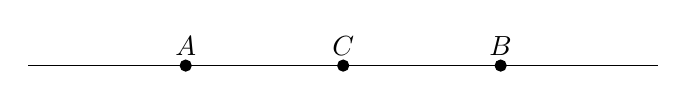
\begin{tikzpicture}
		\draw (-4,0) -- (4,0);
		\filldraw[black] (-2,0) circle[radius = 2pt] node[above] {$A$}; 
		\filldraw[black] (0,0) circle[radius = 2pt] node[above] {$C$};
		\filldraw[black] (2,0) circle[radius = 2pt] node[above] {$B$};
	\end{tikzpicture}
	\i \hspace*{150pt}
	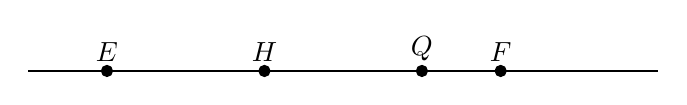
\begin{tikzpicture}
		\draw (-4,0) -- (4,0);
		\filldraw[black] (-3,0) circle[radius = 2pt] node[above] {$E$}; 
		\filldraw[black] (-1,0) circle[radius = 2pt] node[above] {$H$};
		\filldraw[black] (1,0) circle[radius = 2pt] node[above] {$Q$};
		\filldraw[black] (2,0) circle[radius = 2pt] node[above] {$F$};
	\end{tikzpicture}
	\i \hspace*{150pt}
	\begin{tikzpicture}
		
	\end{tikzpicture}
	\i \hspace*{150pt}
	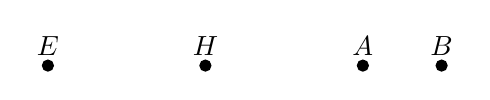
\begin{tikzpicture}
		\filldraw[black] (-3,0) circle[radius = 2pt] node[above] {$E$}; 
		\filldraw[black] (-1,0) circle[radius = 2pt] node[above] {$H$};
		\filldraw[black] (1,0) circle[radius = 2pt] node[above] {$A$};
		\filldraw[black] (2,0) circle[radius = 2pt] node[above] {$B$};
	\end{tikzpicture}
	\end{loigiaichuong}
\end{bt}
\begin{bt}
	\begin{enumerate}[a),leftmargin=*]
		\i Điền kí hiệu $\in ,\notin .$
		\begin{align*}
			&N \quad\square\quad n && B \quad\square\quad m\\
			&N \quad\square\quad p && A \quad\square\quad q\\
			&A \quad\square\quad n && C \quad\square\quad q
		\end{align*}
		\begin{center}
			\begin{tikzpicture}
				
			\end{tikzpicture}
		\end{center}
		\i Gọi tên bộ ba điểm thẳng hàng, bộ ba điểm không thẳng hàng.
	\end{enumerate}
	\begin{loigiaichuong}
		
	\end{loigiaichuong}
\end{bt}
\begin{bt}
	Kể những hình ảnh trong thực tế về hai đường thẳng song song, hai đường thẳng cắt nhau.
	\begin{loigiaichuong}
		
	\end{loigiaichuong}
\end{bt}
\begin{bt}
	Cho hình vẽ sau: 
	\begin{enumerate}[a),leftmargin=*]
		\i Đường nào đi qua$M$mà không đi qua$N$.
		\i Đường nào đi qua$N$mà không đi qua$M$.
		\i Đường nào đi qua cả hai điểm$M,N$.
	\end{enumerate}
	\begin{loigiaichuong}
		
	\end{loigiaichuong}
\end{bt}
\begin{bt}
	Vẽ ba đường thẳng $a,b,c$ sao cho số giao điểm mà chúng có tất cả là:
	
		\begin{tabular}{p{0.25\textwidth} p{0.25\textwidth} p{0.25\textwidth} p{0.25\textwidth}}
			a) 0 & b) 1 &c) 2& d) 3
		\end{tabular}
	\begin{loigiaichuong}
		
	\end{loigiaichuong}
\end{bt}
\begin{bt}
	Cho điểm $P$ không nằm trên đường thẳng $MN$.
	\begin{enumerate}[a),leftmargin=*]
		\i Vẽ tia $Px$ cắt $MN$ tại $A$ nằm giữa $M$ và $N$.
		\i Vẽ tia $Py$ cắt đường thẳng $MN$ tại điểm $B$ sao cho$ N$ nằm giữa $M $và $B$.
		\i Vẽ tia $Pz$ cắt đường thẳng $MN$ tại điểm $C$ sao cho $C$ và $N$ nằm khác phía đối với $M$.
	\end{enumerate}
	\begin{loigiaichuong}
		
	\end{loigiaichuong}
\end{bt}
\begin{bt}
	Cho bốn điểm $A,B,C,D$ kẻ các đoạn thẳng có mặt là 2 trong 4 điểm đó. Có bao nhiêu đoạn thẳng? Hãy kể tên chúng.
	\begin{loigiaichuong}
		
	\end{loigiaichuong}
\end{bt}
\begin{bt}
	Quan sát hình dưới đây và cho biết:
	\begin{enumerate}[a),leftmargin=*]
		\i Có tất cả bao nhiêu tia? Nêu tên các tia đối?
		\i Điểm B nằm trên các tia nào? Tia đối của chúng là tia nào?
		\i Tia $AC$ và tia $CA$ có phải là hai tia đối nhau không?
	\end{enumerate}
	\begin{loigiaichuong}
		
	\end{loigiaichuong}
\end{bt}
\begin{bt}
	Em hãy vẽ 7 điểm trên 1 tờ giấy trắng sao cho có thể kẻ được 6 đường thẳng mà mỗi đường thẳng đều đi qua 3 trong 7 điểm đó. 
	\begin{loigiaichuong}
		
	\end{loigiaichuong}
\end{bt}
\begin{bt}
	Cho hình vẽ bên. Có bao nhiêu điểm là giao điểm của đúng 2 đường.
	\begin{loigiaichuong}
		
	\end{loigiaichuong}
\end{bt} 
\subsubsection*{Mức độ nâng cao}
\begin{bt}
	Cho 2022 điểm phân biệt trong đó không có 3 điểm nào thẳng hàng. Hỏi có bao nhiêu đường thẳng khác nhau đi qua 2 trong 2022 điểm đã cho.
	\begin{loigiaichuong}
		
	\end{loigiaichuong}
\end{bt}
\begin{bt}
	Cho 1998 điểm phân biệt trong đó chỉ có đúng 5 điểm thẳng hàng. Hỏi có bao nhiêu đường thẳng khác nhau đi qua 2 trong 1998 điểm đã cho.
	\begin{loigiaichuong}
		
	\end{loigiaichuong}
\end{bt}
\begin{bt}
	Cho $n$ đường thẳng phân biệt, trong đó bất cứ hai đường thẳng nào cũng cắt nhau, không có 3 đường thẳng nào đồng quy. Biết số giao điểm tạo thành là 780 giao điểm. Tính số đường thẳng.
	\begin{loigiaichuong}
		
	\end{loigiaichuong}
\end{bt}
\begin{bt}
	Cho 1015 đường thẳng cắt nhau trong đó có 15 đường đồng quy. Hỏi có tất cả bao nhiêu giao điểm được tạo thành từ các đường thẳng đó?
	\begin{loigiaichuong}
		
	\end{loigiaichuong}
\end{bt}
\begin{bt}
	Một nhà mạng viễn thông muốn thiết lập mạng điện thoại kết nối giữa hai đội Thái Bình Dương và Đại Tây Dương. Để thuận tiện, mỗi người trong đội này có thể gọi trực tiếp cho tất cả các thành viên trong đội còn lại. Để tiết kiệm, các thành viên trong cùng 1 đội không được kết nối điện thoại với nhau. Bên Thái Bình Dương có 5 thành viên, đội Đại Tây Dương có 8 thành viên. Hỏi nhà mạng phải thiết lập tất cả bao nhiêu đường dây.
	\begin{loigiaichuong}
		
	\end{loigiaichuong}
\end{bt}
\begin{bt}
	Em hãy nêu cách trồng cây thẳng hàng với mỗi trường hợp sau: 
	\begin{enumerate}[a),leftmargin=*]
		\i Hãy trồng 5 cây thành 2 hàng, mỗi hàng có 3 cây.
		\i Hãy trồng 7 cây thành 6 hàng, mỗi hàng có 3 cây.
		\i Hãy trồng 9 cây thành 8 hàng, mỗi hàng 3 cây.
	\end{enumerate}
	\begin{loigiaichuong}
		
	\end{loigiaichuong}
\end{bt}
E. Hướng dẫn giải
Bài 1. 
 


Bài 2. a)
$\begin{align}
	Bài 3.   & N\,\,n \\ 
	Bài 4.  & B\,\,\,m \\ 
	Bài 5.  & N\,\,p \\ 
	Bài 6.  & A\,\,\,q \\ 
	Bài 7.  & A\,\,\,n \\ 
	Bài 8.  & C\,\,\,q \\ 
	Bài 9. \end{align}$
b) Bộ ba điểm thẳng hàng: $M,A,B$.
Bộ ba điểm không thẳng hàng: $M,A,C;M,A,N;A,B,N;A,B,C;C,B,N.$
Bài 10. 
- Hình ảnh về 2 đường thẳng song song: 2 mép bàn, các đường dây điện, song sắt, đường ray tàu hoả, vạch kẻ đường,…

- Hình ảnh về 2 đường thẳng cắt nhau: Cái kéo, 2 mép tường, Tia laser, các con đường giao thông,…

Bài 11. 
a) Đường thẳng $a$ đi qua $M$và không đi qua $N.$
b) Đường thẳng $b$đi qua $Q$ và không đi qua $M.$
c) Đường thẳng $c$đi qua cả hai điểm$M,N.$
Bài 12. 
a) 

b) 

c) 

d) 

Bài 13. 
a) 

b)                

c)

Bài 14. Có 6 đoạn thẳng có mút là 2 trong 4 điểm $A,B,C,D:$
Đoạn thẳng $AB,AC,A\text{D},BC,B\text{D},C\text{D}.$
Bài 15. 
a) Có tất cả 8 tia: $Ax,Ay,Bx,By,Cx,Cy,Dx,Dy.$
b) Điểm $B$ nằm trên tia $Ax,Bx,By.$
Tia đối của tia $Ay$là tia $Ax$.
Tia đối của tia $Ax$là tia $Ay$.
Tia đối của tia $Bx$là tia $Bx$.
Tia đối của tia $By$là tia $B\text{x}$.
c) Hai tia $AC$ và tia $CA$ không là hai tia đối nhau
Bài 16. Ta có thể vẽ như sau: 

Bài 17. Có 10 điểm là giao điểm của đúng 2 đường: $A,B,C,D,E,M,N,O,P,Q.$
Bài tập nâng cao
Bài 18. Do cứ 2 điểm thì tạo thành 1 đường thẳng và không có 3 điểm nào thẳng hàng nên 2022 điểm sẽ nối được với 2021 điểm và mỗi đường thẳng sẽ bị trùng nên ta có: 
Số đường thẳng được tạo thành là: $\frac{2022.2021}{2}=2043231$ (đường thẳng)
Vậy tạo thành được 2043231 đường thẳng khác nhau có đầu mút là 2 trong 2022 điểm đã cho.
Bài 19. Giả sử 1998 điểm phân biệt không có 3 điểm nào thẳng hàng, khi đó: 
Số đường thẳng được tạo thành là: $\frac{1998.(1998-1)}{2}=1995003$(đường thẳng)
5 điểm thẳng hàng tạo thành 1 đường thẳng.
5 điểm không thẳng hàng tạo thành $\frac{5.4}{2}=10$ (đường thẳng)
Số đường thẳng bị giảm đi là: $10-1=9$ (đường thẳng)
Vậy có tất cả: $1995003-9=1994994$ (đường thẳng)
Bài 20. Do cứ 2 điểm thì tạo thành 1 đường thẳng và không có 3 đường thẳng nào đồng quy nên cứ mỗi đường thẳng sẽ giao với $n-1$ đường thẳng và tạo ra $n-1$ giao điểm 
Vậy với $n$ đường thẳng cắt nhau có số giao điểm là: $\frac{n(n-1)}{2}$ (do số giao điểm bị trùng)
Theo đề ra: $\frac{n(n-1)}{2}=780$
$\Leftrightarrow n(n-1)=1560$
Do $40.39=1560$ nên $n=40$(đường thẳng).
Bài 21. Giả sử 1015 đường cắt nhau trong đó không có 3 đường thẳng nào đồng quy. Khi đó số đường thẳng được tạo thành là: $\frac{1015.1014}{2}=514605$(đường thẳng)
15 đường thẳng đồng quy thì có số giao điểm là 1.
15 đường thẳng không đồng quy thì số giao điểm là: $\frac{15.14}{2}=105$(đường thẳng)
Số giao điểm bị giảm là: $105-1=104$(đường thẳng)
Vậy với 1015 đường thẳng cắt nhau trong đó có 15 đường đồng quy thì có số giao điểm là: $514605-104=514501$(đường thẳng)
Bài 22. Mỗi một thành viên của đội Thái Bình Dương sẽ kết nối với 8 thành viên của đội Đại Tây Dương cần 8 đường dây.
Vậy 5 thành viên của đội Đại Tây Dương kết nối với 8 thành viên của đội Đại Tây Dương cần: $5.8=40$(đường dây)
Bài 23. 
a) 

b) 

c) 

$$

\Closesolutionfile{loigiaichung}